\textbf{Setup.} Two training seeds per variant, 1M decisions each (about 2.8 simulated hours at 100\,Hz), trained on seeds $<10^4$ with $A\sim U(0.02,0.14)$. Evaluation: 30 held-out terrains (seeds $\ge 10^5$) at each of four amplitudes per policy, deterministic actions, 8\,s episodes. Because the policies learned slow, careful driving (0.12--0.22\,m/s, comparable to the $\approx$0.15\,m/s implied by the baseline's reported return), \emph{success} is defined as reaching 1\,m of progress along the target direction without a fall. Fig.~\ref{fig:train} shows the learning curves and Table~\ref{tab:h1} the held-out results.

\begin{figure}[t]
\centering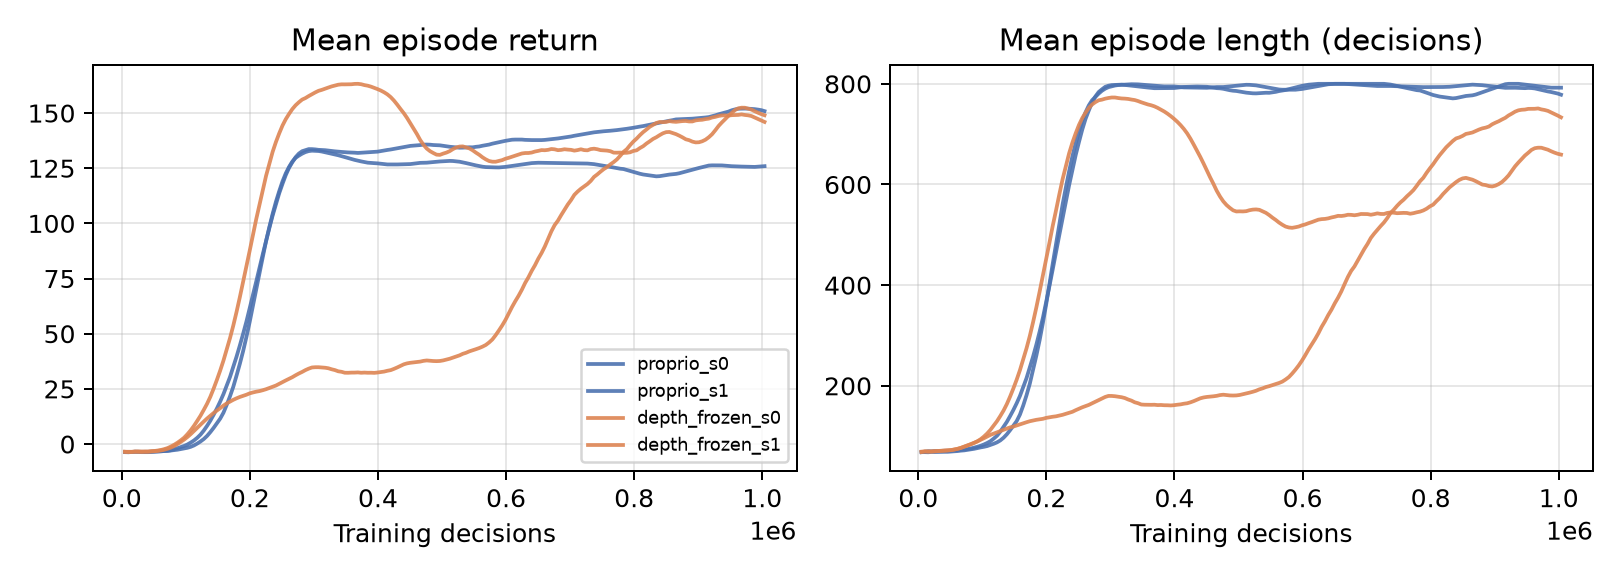
\includegraphics[width=\columnwidth]{figures/training_curves.png}
\caption{Training curves (mean over parallel environments). The drop in episode length after 0.5M decisions for some runs reflects episodes ending early on a fall or on reaching the 2\,m training goal.}\label{fig:train}
\end{figure}

\begin{table*}[t]
\centering\caption{H1: held-out terrains (clean depth). Success and fall rates in \% with 95\% Wilson intervals; pooled over training seeds. Time-to-goal is the mean over successful episodes.}\label{tab:h1}
\small\begin{tabular}{clcccrc}\toprule
Amplitude & Policy & $n$ & Success [\%] & Fall [\%] & Return & TTG [s]\\\midrule
0.04 & Prop.+depth & 60 & 100 [94, 100] & 0 [0, 6] & 168.4 & 4.6 \\
0.04 & Proprio & 60 & 55 [42, 67] & 0 [0, 6] & 145.0 & 5.3 \\
0.08 & Prop.+depth & 60 & 100 [94, 100] & 0 [0, 6] & 166.7 & 4.7 \\
0.08 & Proprio & 60 & 60 [47, 71] & 0 [0, 6] & 142.2 & 5.7 \\
0.12 & Prop.+depth & 60 & 88 [78, 94] & 12 [6, 22] & 153.0 & 4.9 \\
0.12 & Proprio & 60 & 57 [44, 68] & 8 [4, 18] & 126.5 & 6.0 \\
0.18 & Prop.+depth & 60 & 23 [14, 35] & 68 [56, 79] & 81.4 & 5.4 \\
0.18 & Proprio & 60 & 33 [23, 46] & 27 [17, 39] & 103.5 & 6.7 \\
\bottomrule\end{tabular}\end{table*}


\begin{figure}[t]
\centering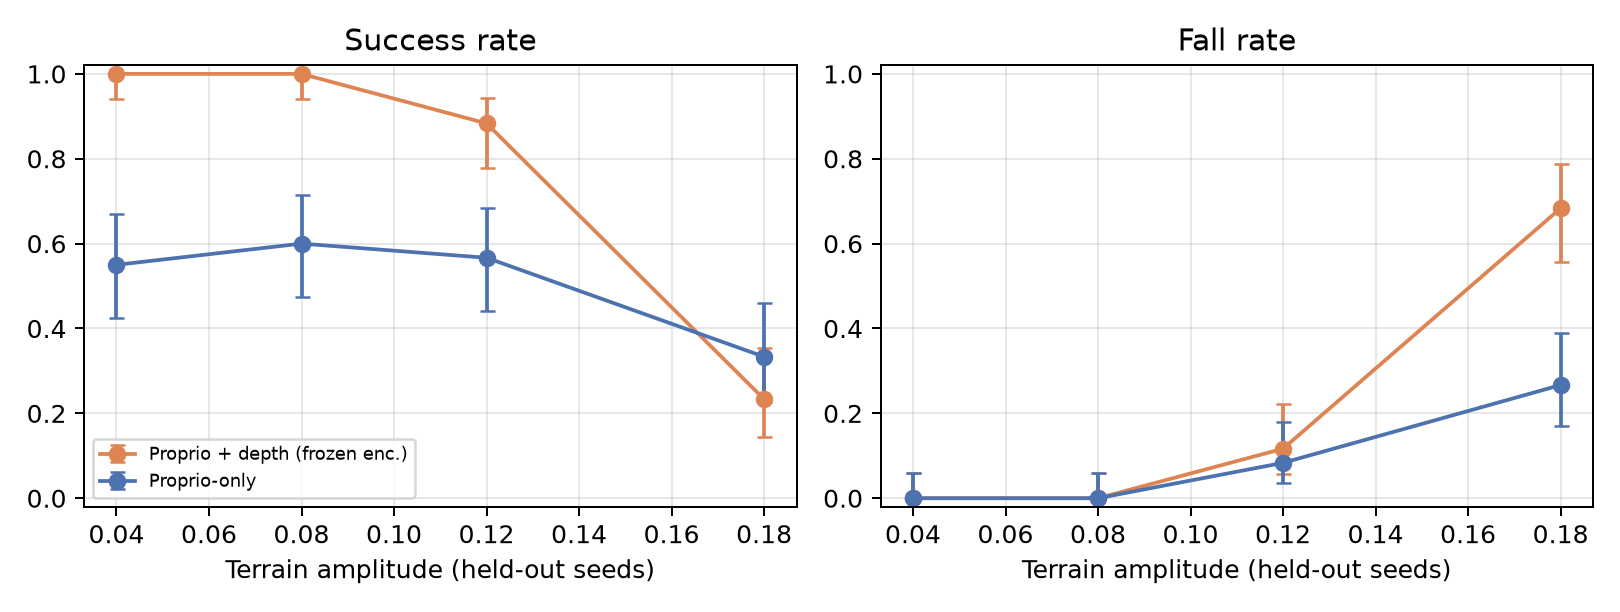
\includegraphics[width=\columnwidth]{figures/h1_success_fall.png}
\caption{H1: success and fall rate versus terrain amplitude (95\% Wilson intervals, pooled over two training seeds).}\label{fig:h1}
\end{figure}

\textbf{Result.} Pooled over the held-out terrains, the proprioception$+$depth policies reach the 1\,m goal more often than proprioception-only (paired difference $+0.27$, 95\% CI $[0.20,0.33]$, Wilcoxon $p<0.001$; Table~\ref{tab:tests}), but they also fall \emph{more} often ($+0.11$, CI $[0.06,0.17]$), mainly on the steepest terrain ($A{=}0.18$: 68\% vs.\ 27\% falls). The per-run breakdown shows that the pooled success gain is driven by a single slow policy: proprioception-only seed~0 succeeds on 85\% of episodes (depth seeds: 80\% and 76\%), whereas proprioception-only seed~1 learned a much slower gait (0.11\,m/s) and succeeds on only 18\%. Per-run mean falls are 11\%/7\% (proprio) vs.\ 16\%/24\% (depth). Hence H1 is \textbf{not supported}: with equal training budget, adding the frozen depth features did not reduce falls and did not give a reliable success benefit; the two-seed pooled test is dominated by seed variance and should be read as such.

\begin{table*}[t]
\centering\caption{Paired comparisons over identical held-out terrains (mean difference, bootstrap 95\% CI, Wilcoxon signed-rank $p$).}\label{tab:tests}
\scriptsize\begin{tabular}{lcccc}\toprule
Test & $n$ & $\Delta$ & 95\% CI & $p$\\\midrule
H1 success: depth frozen - proprio & 120 & +0.267 & [+0.196, +0.329] & <0.001 \\
H1 fell: depth frozen - proprio & 120 & +0.113 & [+0.058, +0.167] & <0.001 \\
H1 return: depth frozen - proprio & 120 & +13.107 & [+6.848, +19.295] & <0.001 \\
H2 success: depth frozen blank - clean & 60 & +0.008 & [-0.017, +0.042] & 0.564 \\
H2 success: depth frozen dropout 0.2 - clean & 60 & +0.008 & [+0.000, +0.025] & 0.317 \\
H2 success: depth frozen noise 0.05 - clean & 60 & +0.000 & [+0.000, +0.000] & 1.000 \\
H2 success: depth frozen noise 0.15 - clean & 60 & +0.000 & [+0.000, +0.000] & 1.000 \\
H2 success: depth frozen noise 0.30 - clean & 60 & +0.008 & [+0.000, +0.025] & 0.317 \\
H2 success: depth frozen occlusion 0.25 - clean & 60 & +0.000 & [+0.000, +0.000] & 1.000 \\
H2 success: depth frozen occlusion 0.50 - clean & 60 & +0.008 & [+0.000, +0.025] & 0.317 \\
H3 success: goal direction - goal relative & 90 & +0.000 & [+0.000, +0.000] & 1.000 \\
\bottomrule\end{tabular}\end{table*}

